
\documentclass[twocolumn]{article}
\usepackage{mathpazo}
\usepackage{microtype}
\usepackage{times}
\usepackage{titlesec} % 1
%\usepackage{sectsty} % "제 1 절" ...

 %%%%%%%%%%%%%%%%%%%%%%%%%%%%%%%%%%%%%%%%%%%%%%%%%%%%%%%%%%%%%%%%%%%%%%%%%%%%%
 %                              My Commands
\newcommand{\bi}{\begin{itemize}}
\newcommand{\ei}{\end{itemize}}
\newcommand{\be}{\begin{enumerate}}
\newcommand{\ee}{\end{enumerate}}
\newcommand{\ii}{\item}
\newtheorem{Def}{Definition}
\newtheorem{Lem}{Lemma}
\usepackage{algorithm}
\usepackage{algorithmicx}
\usepackage{algpseudocode}

\usepackage{graphicx}
\graphicspath{%
        {converted_graphics/}
        {./images/}
}

\usepackage{color}
\usepackage{xcolor}
\usepackage{listings}
\usepackage{caption}
\DeclareCaptionFont{white}{\color{white}}
\DeclareCaptionFormat{listing}{\colorbox{gray}{\parbox{\textwidth}{#1#2#3}}}
\captionsetup[lstlisting]{format=listing,labelfont=white,textfont=white}
\usepackage{verbatimbox}

\usepackage[hangul,nonfrench,finemath]{kotex}
    
\setlength\textwidth{7in} 
\setlength\textheight{9.5in} 
\setlength\oddsidemargin{-0.25in} 
\setlength\topmargin{-0.25in} 
\setlength\headheight{0in} 
\setlength\headsep{0in} 
%\setlength\columnsep{5pt}
\sloppy 
 
\begin{document}

\title{
\vspace{-0.5in}\rule{\textwidth}{2pt}
\begin{tabular}{ll}\begin{minipage}{4.75in}\vspace{6px}
\noindent\large {\it KIWI Project}@Data Management Research Section\\
\vspace{-12px}\\
\noindent\LARGE ETRI\qquad  \large Technical Report 15ZS1410-TR-63
\end{minipage}&\begin{minipage}{2in}\vspace{6px}\small
218 Gajeong-ro, Yuseong-gu\\
Daejeon, 305-700, South Korea\\
http:/$\!$/www.etri.re.kr/\\
http:/$\!$/sungsoo.github.com/\quad 
\end{minipage}\end{tabular}
\rule{\textwidth}{2pt}\vspace{0.25in}
\LARGE \bf 논문 리뷰: 드레멜 - 웹스케일 데이터셋에 대한 인터랙티브 분석 \\
\large Paper Review: Dremel - Interactive Analysis of Web-Scale Dataset
}

\date{}

\author{
{\bf Sung-Soo Kim}\\
\it{sungsoo@etri.re.kr}
}

\maketitle

\begin{abstract}
SQL온하둡 (SQL-on-Hadoop)은 하둡분산파일시스템(HDFS)에 저장된 데이터를 많은 데이터 과학자에게 익숙한 표준SQL 언어로 빠르게 조회하게 해주는 기술이다. 
이 기술을 통해 하둡 환경의 데이터를 기존 데이터 웨어하우스처럼 SQL 방식으로 들여다볼 수 있게 해준다. 
맵리듀스와 하이브QL의 단점을 개선하고 기존 DW시스템에 준하는 성능을 제공하는 것이 SQL온하둡의 궁극적인 목표다.

본 기술문서에서는 SQL온하둡의 시초라 볼 수 있는 구글의 드레멜 논문을 리뷰한다.  그럼 왜 이 논문을 리뷰해야 하는가?
그 이유는 구글에서 기존 맵리듀스에서 얻을 수 없었던 웹스케일 데이터에 대한 인터랙티브 분석을 위해 제시한 기술이 무엇이며, 어떠한 장단점이 있는 지 이해하는 것이 KIWI 과제 연구개발에 도움을 줄 수 있기 때문이다. 
드레멜의 주요한 연구동기, 공헌, 문제해결법, 그리고 장단점 중심으로 설명하고 있다.
\end{abstract}

\section{Introduction}
Dremel is a distributed system developed at Google for interactively querying large datasets and powers Google's BigQuery service \cite{Melnik:2011}. Google Dremel is the inspiration for Apache Drill project.
\bi
\ii \textit{Near real time interactive analysis} (instead batch processing). SQL-like query language.
\ii \textit{Nested data} (most of unstructured data supported) with a column storage representation.
\ii \textit{Tree architecture} (as in web search): multi-level execution trees for query processing.
\ei

\subsection{Motivation}
The main motivation of the paper is the inability of existing big data infrastructure (MapReduce-BigTable and Hadoop) to perform \textit{fast ad-hoc explorations/queries} into web-scale data-sets. 
In this context, ad-hoc explorations/queries mean \textit{on-the-fly} queries, which are issued by users when they need it. The execution time of ad-hoc queries is expected to be fast so that users can \textit{interactively} explore the datasets.

Secondary motivation of the paper is the needs of more \textit{user-friendly query mechanism} to make data analytic in big data infrastructure easier and faster. 
Pig and Hive try to solve this challenge by providing SQL-like query language in Hadoop, 
but they only solve the \textit{usability} issue and \textit{not} the \textit{performance} issue.
Solving these issues allows faster, more efficient and more effective data analytic in big data infrastructure 
which implies higher productivity for data scientists and engineers who are working in big data analytic. 
Therefore, these issues are interesting and important to be solved.

\section{Contributions}
The main contribution of Dremel is\textit{ high-performance} technique in processing web-scale data-set for 
ad-hoc query usage. The mechanism solves these following challenges:

\be
\ii \textit{Inefficiency in storing data for ad-hoc query.}
Ad-hoc queries most of the time do not need all the available field/column in a table. Therefore the authors propose columnar data model that improve data retrieval performance. It was novel solution because well-known big data processing platforms (such as MapReduce on Hadoop) work at record-structure data model at that time.
\ii \textit{Performance and scalability challenge in processing the data.}
Multi-level serving tree model allows high parallelism in processing the data. It also allows optimization of query in each of the tree level. Query scheduling allows prioritization of the execution. Both techniques solve performance challenge in data processing.
Scalability challenge is also solved since we can easily add more nodes to process more data in multi-level serving tree model. Separation of query scheduler from root server is good because it decouples query scheduling responsibility with job tracking (note that: job tracking is performed by root server). This scheduler model implies higher scalability when the number of leaf servers is huge.
\ee
The minor contribution of this paper is the use of actual Google data set in the experiment. 
This usage gives other researchers insight on the practical magnitude of web-scale data-sets.

\section{Solutions}
Why Dremel can be so drastically fast? 
The answer can be found in two important innovations which gives Dremel this unprecedented performance:
\be
\ii \textbf{Columnar Storage.} Data is stored in a columnar storage fashion which makes possible to achieve very high compression ratio and scan throughput.
\ii \textbf{Tree Architecture} is used for dispatching queries and aggregating results across thousands of machines in a few seconds.
\ee

\subsection{Columnar Data Model}
As mentioned before, ad-hoc queries only need small subset of fields/columns in tables. \textit{Record-structure} data model introduces significant inefficiencies. The reason is in order to retrieve the needed fields/columns, we need to read the whole record data, including unnecessary fields/columns. To reduce these inefficiencies, \textit{columnar data model} is introduced. Columnar data model allows us to read only the needed fields/columns for ad hoc queries. This model will reduce the data retrieval inefficiencies and increase the speed. The authors also explain how to convert from record-structure data model to columnar model and vice versa.

\begin{figure}[htb]
        \centering
        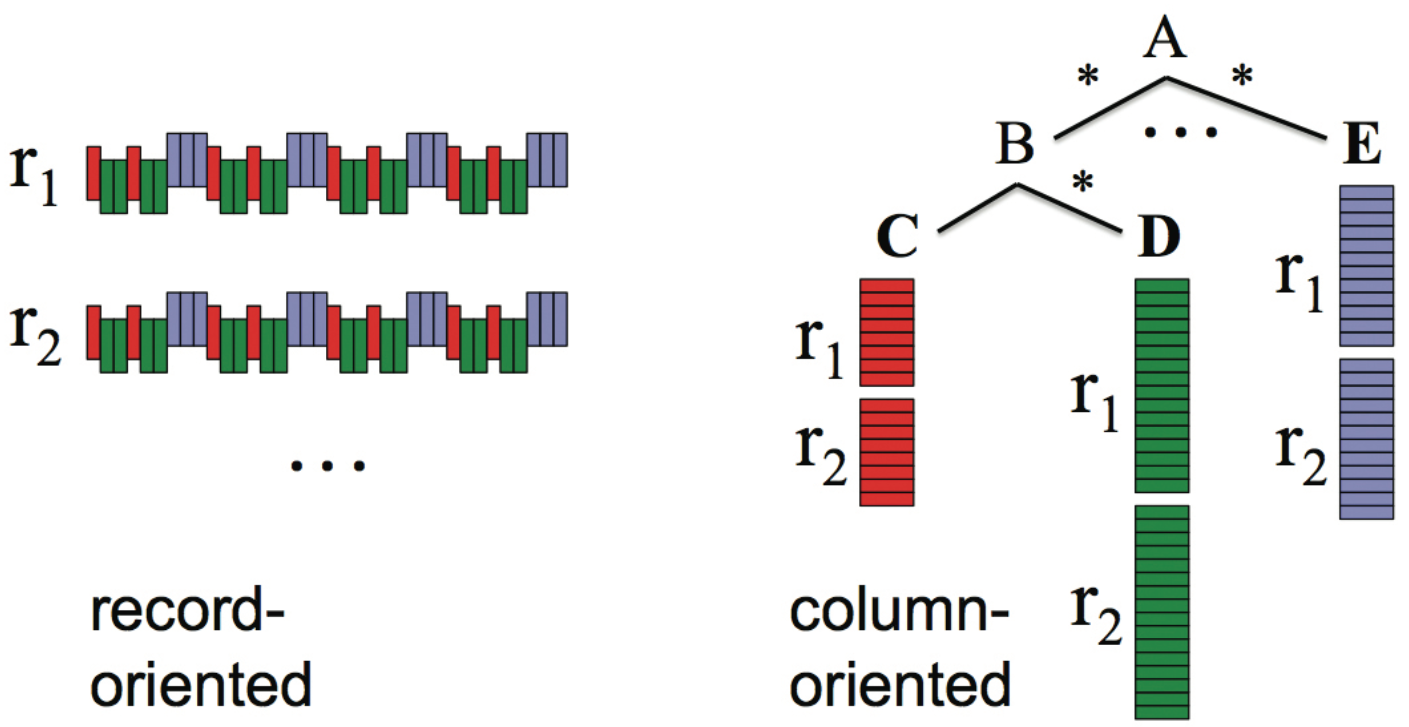
\includegraphics[width=0.45\textwidth]{column-oriented.png}
        \caption{Columnar storage of Dremel}
        \label{fig:column-oriented}
\end{figure}

\subsection{Multi-level Serving Tree}
The authors use \textit{multi-level serving tree} in columnar data processing. Typical multi-level serving tree consists of a root server, several intermediate servers and many leaf servers as shown in Figure \ref{fig:tree}. There are two reasons behind multi-level serving tree:
\be
\ii \textit{Characteristics of ad hoc queries} where the result set size is small or medium. The overhead of processing these kinds of data in parallel is small.
\ii \textit{High degree of parallelism} to process small or medium-size data.
\ee
\begin{figure}[htb]
        \centering
        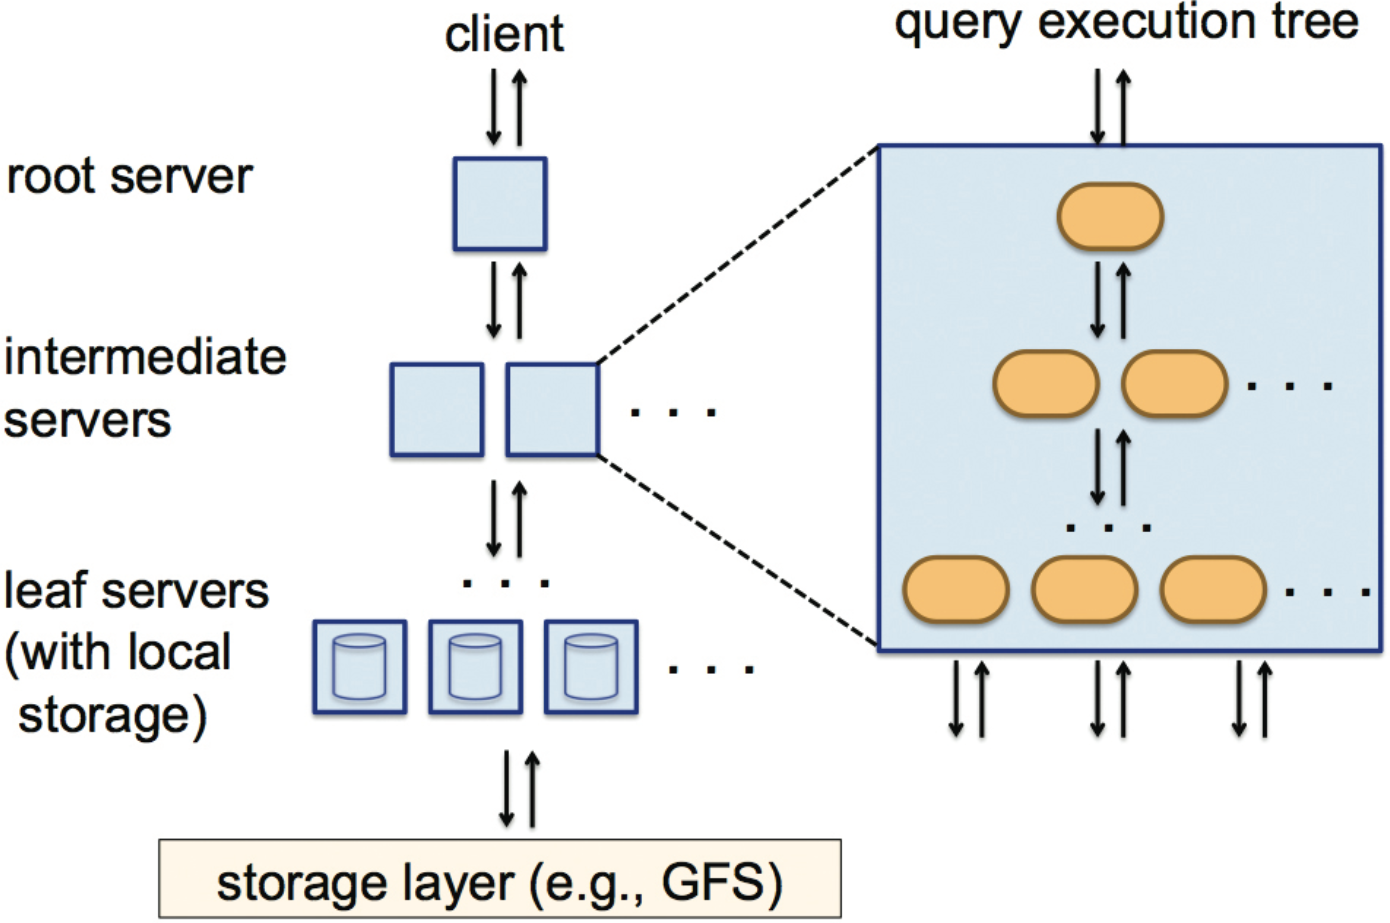
\includegraphics[width=0.45\textwidth]{query-execution-tree.png}
        \caption{Tree architecture of Dremel}
        \label{fig:tree}
\end{figure}

By leveraging this architecture, Google was able to implement the distributed design for Dremel and realize the vision of the \textit{massively parallel columnar-based database} on the cloud platform.

\subsection{Query Dispatcher}
The authors propose a mechanism to regulate resource allocation for each leaf servers and the mechanism is handled by module called query dispatcher. Query dispatcher works in slot (number of processing unit available for execution) unit. It allocates appropriate number of tablets into their respective slot. It deals with stragglers by moving the tablets from slow straggler slots into new slots.

\subsection{SQL-like query}
People with SQL background can easily use Dremel to perform data analytics in web-scale datasets. Unlike Pig and Hive, Dremel does not convert SQL-like queries into MapReduce jobs, therefore Dremel should have faster execution time compared to Pig and Hive.

\begin{figure}[htb]
        \centering
        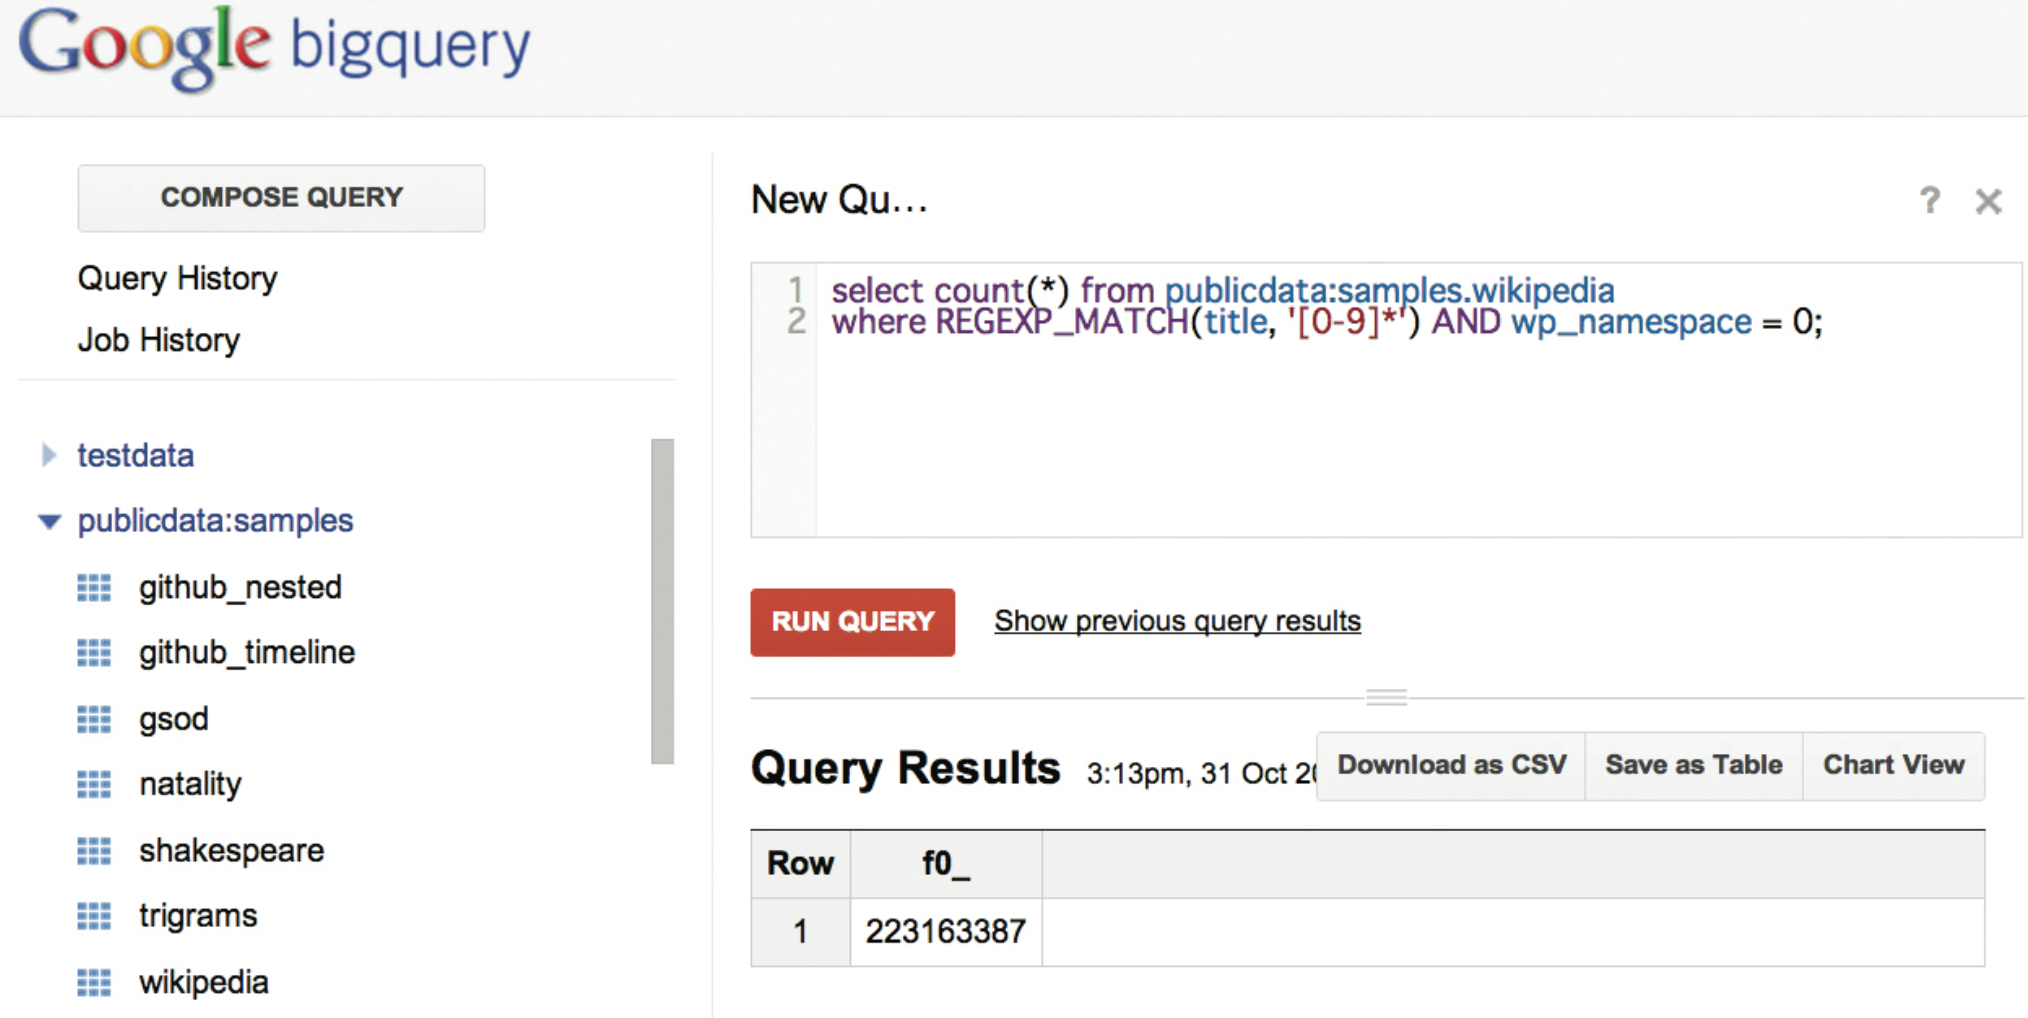
\includegraphics[width=0.45\textwidth]{google-bigquery.png}
        \caption{Google BigQuery}
        \label{fig:bigquery}
\end{figure}

BigQuery provides the core set of features available in Dremel to third party developers \cite{Sato:2012}. It does so via a REST API, command line interface, Web UI, access control, data schema management and the integration with Google Cloud Storage.

BigQuery and Dremel share the same underlying architecture and performance characteristics. Users can fully utilize the power of Dremel by using BigQuery
to take advantage of Google’s massive computational infrastructure. This incorporates valuable benefits like multiple replication across regions and
high data center scalability. Most importantly, this infrastructure requires no management by the developer.


\subsection{BigQuery versus MapReduce}
Google has been using MapReduce for Big Data processing for quite some time, and unveiled this in a research paper2 in December of 2004. Some readers may have heard about this product, and its open source implementation Hadoop, and may wonder about the difference between the two. This is the difference:
\bi
\ii Dremel is designed as an interactive data analysis tool for large datasets 
\ii MapReduce is designed as a programming framework to batch process large datasets
\ei
Moreover, Dremel is designed to finish most queries within seconds or tens of seconds and can even be used by non-programmers, whereas MapReduce takes much longer (at least minutes, and sometimes even hours or days) to finish processing a dataset query.

\section{Strong Points}
\be
\ii Identification of the characteristics of ad-hoc queries data set.
The authors correctly identify the main characteristic of data set returned from ad-hoc queries, which is: only small number of fields are used by ad hoc-queries. This finding allows the authors to develop columnar data model and use multi-level serving tree to process the columnar data model.
\ii Fast and lossless conversion between nested record structure model and columnar data model.
Although columnar data model has been used in other related works, the fast and lossless conversion algorithm that the authors propose is novel and one of the key contributions of Dremel.
\ii Magnitude and variety of datasets for experiments.
The magnitude of datasets is huge and practical. These magnitude and variety of data-sets increase the confirming power of Dremel solution and proof its high performance.
\ee
\section{Weak Points}
\be
\ii Record-oriented data model can still outperform columnar data model. This is the main shortcoming of Dremel, however credit must be given on the authors since they do not hide this shortcoming and they provide some insight on this shortcoming.
\ii Performance analysis on the \textit{data model conversion} is not discussed. They claim that the conversion is fast, but they do not support this argument using experiment data.
\ii "Cold" setting usage in Local Disk experiment. In Local Disk experiment, the authors mention that "\textit{all reported times are cold}". Using cold setting in database or storage benchmarking is not recommended because the data is highly \textit{biased} with disk access performance. When the database is "cold", query execution performance in the start of the experiment will highly depend on the disk speed. In the start of the experiment, most of the operations involve moving data from disk to OS cache, and the execution performance will be dominated by disk access.
\ee

\section{Conclusion}
BigQuery is a query service that allows you to run SQL-like queries against multiple terabytes of data in a matter of seconds. 
The technology is one of the Google’s core technologies, like MapReduce and Bigtable, and has been used by Google internally for various analytic tasks since 2006. Google has launched Google BigQuery, an externalized version of Dremel. BigQuery made it possible for developers and enterprises to utilize the power of Dremel for their Big Data processing requirements and accelerate their business at the same swift pace.

While MapReduce is suitable for long-running batch processes such as data mining, BigQuery is the best choice for ad hoc OLAP/BI queries that require results as fast as possible. BigQuery is the cloud-powered massively parallel query database that provides extremely high full-scan query performance and cost effectiveness compared to traditional data warehouse solutions and appliances.

\bibliographystyle{abbrv}
\bibliography{sqlonhadoop}

\end{document}
